\documentclass[12pt]{book}
\usepackage{fontspec}
\setmainfont{TeX Gyre Pagella}
\usepackage[paperwidth=8in,paperheight=8in,margin=0.6in]{geometry}
\usepackage{xcolor}
\usepackage{amssymb}
\usepackage{tikz}
\usetikzlibrary{arrows.meta}
\pagestyle{empty}
\setlength{\parindent}{0pt}

\newcommand{\artnote}[1]{{\color{gray!70}\small\itshape [Illustration: #1]}\par\vspace{0.3in}}
\newcommand{\bigline}[1]{{\Huge #1}\par}
\newcommand{\pagenum}[1]{\vfill{\color{gray!50}\footnotesize #1}}
\newcommand{\sprollpage}{\newpage\vspace*{0.4in}}

\begin{document}

\thispagestyle{empty}
\begin{center}
\vspace*{1.1in}
{\Huge \textbf{SPROLL 10}}\\[0.4in]
{\huge \textbf{Four Moves Make a World}}\\[0.5in]
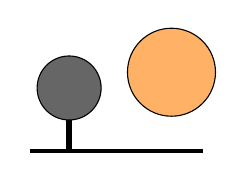
\begin{tikzpicture}
\draw[line width=1.5pt] (-1.1,-0.5) -- (1.1,-0.5);
\filldraw[fill=orange!60] (0.7,0.5) circle (0.22in);
\draw[line width=2pt] (-0.6,-0.5) -- (-0.6,0.1);
\filldraw[fill=black!60] (-0.6,0.3) circle (0.16in);
\end{tikzpicture}
\\[0.4in]
{\large \textit{everything you have, put to use together}}\\[0.3in]
{\small The Sproll Curriculum $\cdot$ Cycle I: Pops}
\end{center}

\sprollpage
\begin{center}
\vspace*{1.5in}
{\Large The Sproll Curriculum}\\[0.2in]
{\normalsize Cycle I --- Pops: Things, Differences, and Counting}\\[0.6in]
{\small Sproll 10 of 40 \quad $\cdot$ \quad follows Sproll 09: Parts With a Past}
\end{center}
\pagenum{2}

\sprollpage
\begin{center}
\vspace*{0.6in}
\artnote{the four small icons from the end of Sproll 09: a dot, a crossed shape, a connecting line, a lens}
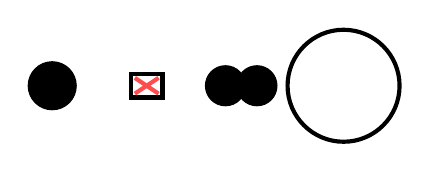
\begin{tikzpicture}
\filldraw[fill=black] (-2.1,0) circle (0.12in);
\draw[line width=1.5pt] (-1.1,-0.15) rectangle (-0.7,0.15);
\draw[line width=1.5pt, red!70] (-1.05,-0.1) -- (-0.75,0.1);
\draw[line width=1.5pt, red!70] (-1.05,0.1) -- (-0.75,-0.1);
\filldraw[fill=black] (0.1,0) circle (0.1in);
\filldraw[fill=black] (0.5,0) circle (0.1in);
\draw[line width=1.5pt] (0.23,0) -- (0.37,0);
\draw[line width=1.5pt] (1.6,0) circle (0.28in);
\end{tikzpicture}
\vspace{0.3in}
\bigline{Pop. Refuse. Bind. Collapse.}\vspace{0.1in}
{\Large Let's build a small world.}
\end{center}
\pagenum{3}

\sprollpage
\begin{center}
\vspace*{0.8in}
\artnote{a plain empty page, ready to begin}
{\color{gray!40}\Huge (an empty world)}
\vspace{0.35in}
\bigline{Pop a sun.}
\end{center}
\pagenum{4}

\sprollpage
\begin{center}
\vspace*{0.8in}
\artnote{an orange sun shape now on the page, with a plain ground line beneath}
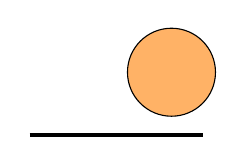
\begin{tikzpicture}
\draw[line width=1.5pt] (-1.1,-0.5) -- (1.1,-0.5);
\filldraw[fill=orange!60] (0.7,0.3) circle (0.22in);
\end{tikzpicture}
\vspace{0.35in}
\bigline{Pop a tree.}
\end{center}
\pagenum{5}

\sprollpage
\begin{center}
\vspace*{0.7in}
\artnote{the sun and ground, now with a simple tree shape added nearby but not yet connected to the ground}
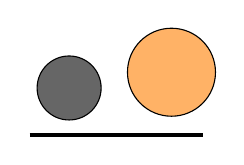
\begin{tikzpicture}
\draw[line width=1.5pt] (-1.1,-0.5) -- (1.1,-0.5);
\filldraw[fill=orange!60] (0.7,0.3) circle (0.22in);
\filldraw[fill=black!60] (-0.6,0.1) circle (0.16in);
\end{tikzpicture}
\vspace{0.35in}
\bigline{Bind the tree to the ground.}
\end{center}
\pagenum{6}

\sprollpage
\begin{center}
\vspace*{0.7in}
\artnote{the tree now connected to the ground line with a small trunk, sun and ground unchanged}
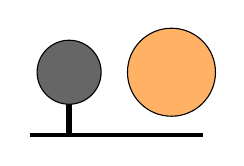
\begin{tikzpicture}
\draw[line width=1.5pt] (-1.1,-0.5) -- (1.1,-0.5);
\filldraw[fill=orange!60] (0.7,0.3) circle (0.22in);
\draw[line width=2pt] (-0.6,-0.5) -- (-0.6,0.1);
\filldraw[fill=black!60] (-0.6,0.3) circle (0.16in);
\end{tikzpicture}
\vspace{0.35in}
\bigline{Now the tree belongs to the ground.}
\end{center}
\pagenum{7}

\sprollpage
\begin{center}
\vspace*{0.6in}
\artnote{the same small scene, with a faint, crossed-out second sun sketched off to the side, not part of the main scene}
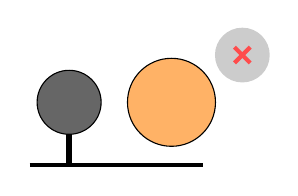
\begin{tikzpicture}
\draw[line width=1.5pt] (-1.1,-0.5) -- (1.1,-0.5);
\filldraw[fill=orange!60] (0.7,0.3) circle (0.22in);
\draw[line width=2pt] (-0.6,-0.5) -- (-0.6,0.1);
\filldraw[fill=black!60] (-0.6,0.3) circle (0.16in);
\draw[fill=orange!60, line width=1pt, gray!40] (1.6,0.9) circle (0.13in);
\draw[line width=1.5pt, red!70] (1.5,0.8) -- (1.7,1.0);
\draw[line width=1.5pt, red!70] (1.5,1.0) -- (1.7,0.8);
\end{tikzpicture}
\vspace{0.3in}
\bigline{Refuse a second sun.}\vspace{0.1in}
{\Large Not this way. One sun is enough.}
\end{center}
\pagenum{8}

\sprollpage
\begin{center}
\vspace*{0.6in}
\artnote{the small world scene, sun ground and tree, framed as a finished picture}
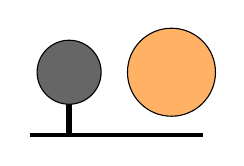
\begin{tikzpicture}
\draw[line width=1.5pt] (-1.1,-0.5) -- (1.1,-0.5);
\filldraw[fill=orange!60] (0.7,0.3) circle (0.22in);
\draw[line width=2pt] (-0.6,-0.5) -- (-0.6,0.1);
\filldraw[fill=black!60] (-0.6,0.3) circle (0.16in);
\end{tikzpicture}
\vspace{0.3in}
\bigline{Rule: what does the world look like?}\vspace{0.1in}
{\Large Collapse to this.}
\end{center}
\pagenum{9}

\sprollpage
\begin{center}
\vspace*{0.6in}
\artnote{the same construction, with a different rule label above and a numeral 2 beneath, since only sun and tree were actually chosen (refused sun does not count)}
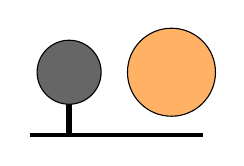
\begin{tikzpicture}
\draw[line width=1.5pt] (-1.1,-0.5) -- (1.1,-0.5);
\filldraw[fill=orange!60] (0.7,0.3) circle (0.22in);
\draw[line width=2pt] (-0.6,-0.5) -- (-0.6,0.1);
\filldraw[fill=black!60] (-0.6,0.3) circle (0.16in);
\end{tikzpicture}
\vspace{0.15in}
{\large Rule: count only the Pops.}
\vspace{0.15in}\\
{\Huge \textbf{2}}
\end{center}
\pagenum{10}

\sprollpage
\begin{center}
\vspace*{0.4in}
\artnote{the full ledger of the build: Pop sun, Pop tree, Bind tree-ground, Refuse second sun, four entries stacked as one history}
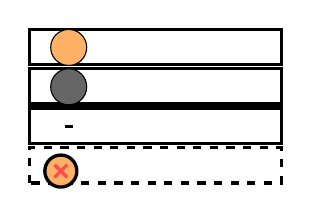
\begin{tikzpicture}
\draw[line width=1.2pt] (-1.6,1.2) rectangle (1.6,1.65);
\filldraw[fill=orange!60] (-1.1,1.42) circle (0.09in);
\draw[line width=1.2pt] (-1.6,0.7) rectangle (1.6,1.15);
\filldraw[fill=black!60] (-1.1,0.92) circle (0.09in);
\draw[line width=1.2pt] (-1.6,0.2) rectangle (1.6,0.65);
\draw[line width=1.2pt] (-1.15,0.42) -- (-1.05,0.42);
\draw[line width=1.2pt, dashed] (-1.6,-0.3) rectangle (1.6,0.15);
\draw[fill=orange!60, line width=1.2pt] (-1.2,-0.15) circle (0.08in);
\draw[line width=1.2pt, red!70] (-1.28,-0.23) -- (-1.12,-0.07);
\draw[line width=1.2pt, red!70] (-1.28,-0.07) -- (-1.12,-0.23);
\end{tikzpicture}
\vspace{0.15in}
\bigline{One record. All four moves.}
\end{center}
\pagenum{11}

\sprollpage
\begin{center}
\vspace*{0.8in}
\artnote{the small world scene once more, calm and complete}
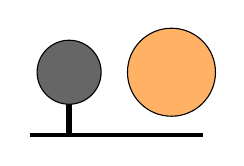
\begin{tikzpicture}
\draw[line width=1.5pt] (-1.1,-0.5) -- (1.1,-0.5);
\filldraw[fill=orange!60] (0.7,0.3) circle (0.22in);
\draw[line width=2pt] (-0.6,-0.5) -- (-0.6,0.1);
\filldraw[fill=black!60] (-0.6,0.3) circle (0.16in);
\end{tikzpicture}
\vspace{0.35in}
\bigline{Four moves. One growing history.}\vspace{0.1in}
{\Large Many worlds you can build.}
\end{center}
\pagenum{12}

\sprollpage
\begin{center}
\vspace*{0.6in}
\artnote{a blank page with just a boundary circle drawn on it, empty inside, as if inviting the next world to be built with a border first}
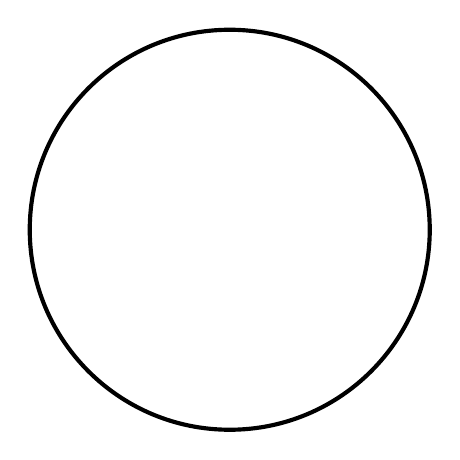
\begin{tikzpicture}
\draw[line width=1.5pt] (0,0) circle (1in);
\end{tikzpicture}
\vspace{0.3in}
\bigline{Every world needs a boundary.}\vspace{0.1in}
{\Large What belongs? What doesn't?}
\end{center}
\pagenum{13}

\sprollpage
\begin{center}
\vspace*{0.7in}
\artnote{a closing image looking back over Cycle I: small versions of all the recurring devices, a dot, a ledger strip, the boundary circle, arranged quietly together}
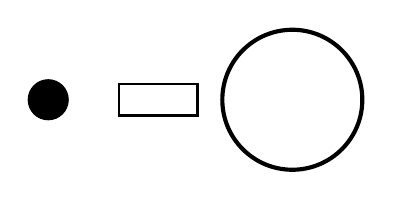
\begin{tikzpicture}
\filldraw[fill=black] (-1.8,0) circle (0.1in);
\draw[line width=1pt] (-0.9,-0.2) rectangle (0.1,0.2);
\draw[line width=1.5pt] (1.3,0) circle (0.35in);
\end{tikzpicture}
\vspace{0.3in}
\bigline{That is Cycle I.}
\vspace{0.3in}
{\small \textit{--- turn the page for Sproll 11: The Box ---}}
\end{center}
\pagenum{14}

\sprollpage
\vspace*{0.3in}
{\large \textbf{A Note for Grown-Ups}}
\vspace{0.2in}

\normalsize
This book introduces no new primitive; its entire purpose is consolidation, using all four Spherepop primitives together in one small, deliberately simple construction. A child who can narrate this book's little world back, in their own words, using the words Pop, Refuse, Bind, and Collapse correctly, has completed Cycle I's actual goal.

\vspace{0.15in}
This closes the historical-construction foundation the rest of the curriculum builds on. Cycle II begins from a genuinely new question, what belongs inside a boundary and what does not, which requires nothing beyond what this book has already established, but organizes it differently: instead of building one history at a time, the child will begin working with many possible Pops at once, some admitted and some not, under a stated rule of membership.

\vspace{0.3in}
{\small Sproll 11: The Box begins Cycle II of the Sproll Curriculum.}
\pagenum{15}

\end{document}
